\documentclass[a5paper]{article}
\usepackage[utf8]{inputenc}
\usepackage[margin = 2cm]{geometry}
\usepackage{graphicx}

\font\domino=domino
\catcode`\^=12 %\offinterlineskip

\title{%
    Conveyor Rummy\\%
    \large A game for 2--4 players\\%
    \normalsize \textit{$\beta$1.0.0}
}

\author{%
    Niko Lepka and Eva Jacobsen\\%
    \footnotesize With help from Alex Laterman%
}
    
\date{July 23 2021}

\newcommand{\aside}{\paragraph{Aside}}
\newcommand{\example}{\paragraph{Example}}
\newcommand{\note}{\paragraph{Note}}
\begin{document}

\begin{center}
  \huge Conveyor Rummy\\
  \Large By Niko Lepka \& Eva Jacobsen\\
  \normalsize \today\\
  \large For 2--4 players, 15--30 min\\
  \footnotesize v1.2.0 - Playtest Version
\end{center}

\noindent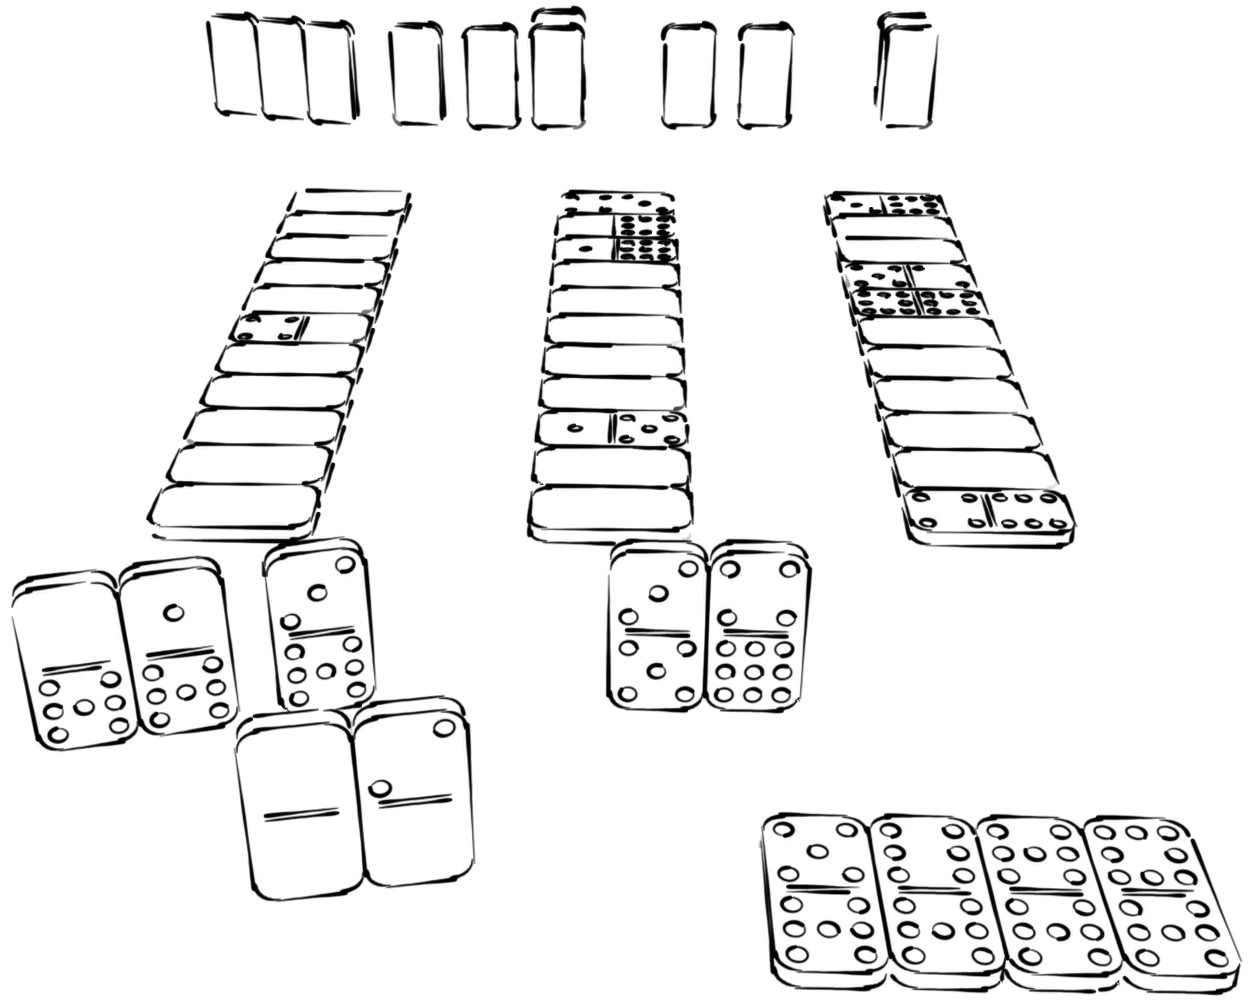
\includegraphics[width = \linewidth]{graphics/dominoes-gameplay.png}

\newpage
\section*{Intro}
Conveyor Rummy is played with dominoes, where the numbers on the tiles serve as both suits and ranks. 
Unlike traditional playing cards or Rummy tiles, the dominoes allow for a more dynamic and flexible gameplay experience. 
With the ability to adapt to your hand's composition seamlessly, you'll be able to strategically outmaneuver your opponents and dominate the game.

\subsection*{Conventions}
This rulebook follows a number of conventions outlined here:

\example Examples are written like this and serves as an aid to better explain a rule.

\note Notes are written like this, and serve to bring edge-cases to the reader's attention.

\aside Asides can be thought of as ``developer commentary'', and exist to bring some insight to \textit{why} a certain rule was implemented the way it was.
\newpage
\tableofcontents
\newpage
\section{Object}
Conveyor Rummy is a rummy-style game played with dominoes.
Over a series of turns, players draw tiles from a number of columns---or ``conveyors'', trying to complete sets and runs---called \textit{melds}.
Whoever gets rid of all their dominoes first wins the round.
\section{Requirements}
\begin{itemize}
    \item A double-9\footnote{If you are unfamiliar with this terminology: ``double-9'' and ``double-12'' simply means that the largest tile in the set is a 9--9 or a 12--12} set of 55 dominoes (2 players)
    \item A double-12 set of 91 dominoes (3-4 players)
    \item Domino stands/racks (optional, but recommended)
    \item A way to keep score---pen and paper is fine
\end{itemize}

\aside Unfortunately in our play-testing, a double-6 set made for extremely quick games, even with just two players. Rounds would be over in just one or two turns. If this is fine with you, do not hesitate to play this variant.
\section{Setup}
Before beginning, players must decide how many rounds to play. 
We recommend 4 rounds for 2 players, and 8 rounds for 3-4 players, but feel free to change it up.
\subsection{2 Players}

\begin{enumerate}
    \item Flip all the dominoes face-down onto the table and give them a good shuffle.
    \item Arrange all the dominoes in 5 columns of 11
    \item Flip over the middle domino in each column.
\end{enumerate}

\subsection{3--4 Players}

\begin{enumerate}
    \item Flip all the dominoes face-down onto the table and give them a good shuffle.
    \item Arrange all the dominoes in 7 columns of 13
    \item Flip over the middle domino in each column.
\end{enumerate}

\begin{figure}[ht]
\centering
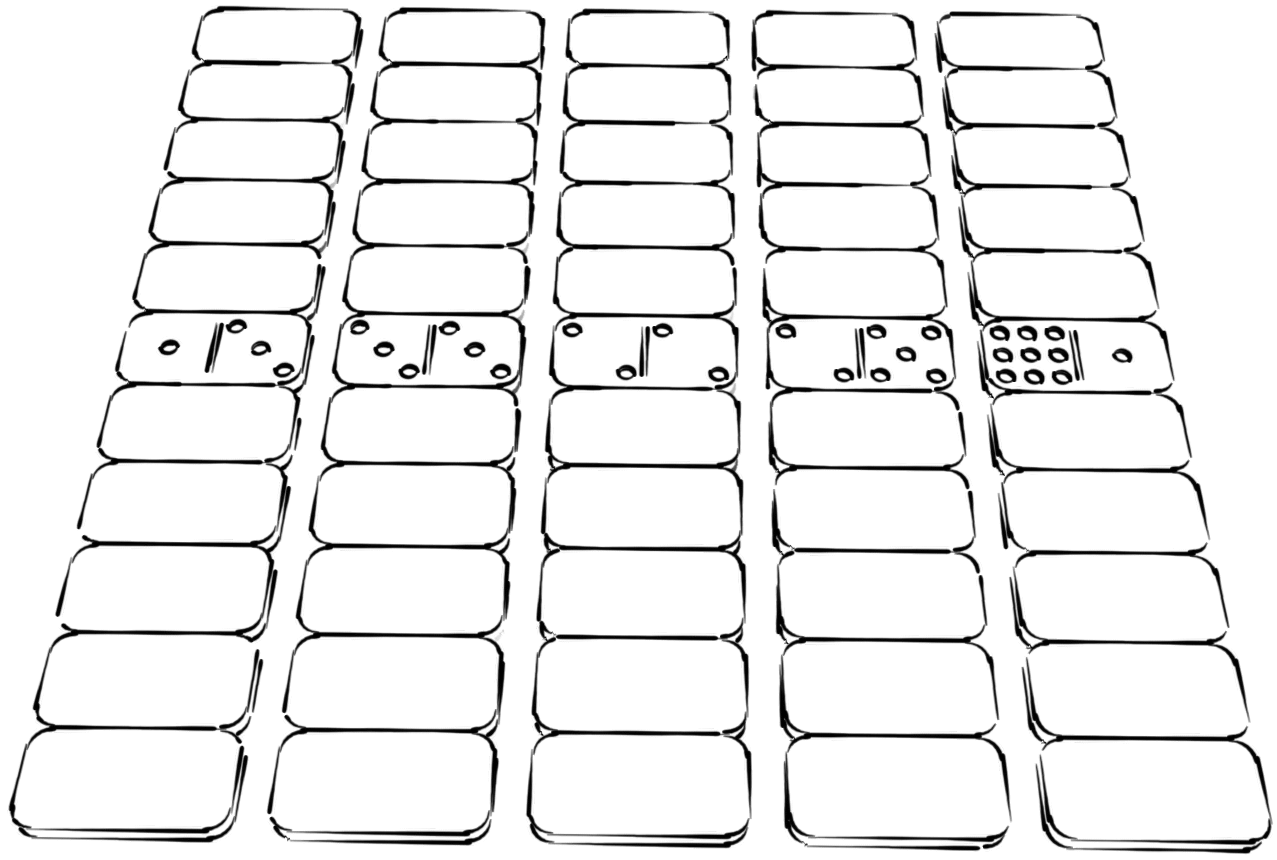
\includegraphics[width = \linewidth]{graphics/dominoes-setup.png}
\caption{Example setup for 2 players. 5 columns of 11 tiles.}
\end{figure}
\subsection{Selection Round}

Proceeding clockwise around the table, starting with the youngest player, a player may choose to either 
\begin{itemize} 
\item Reveal one piece in any column
\item Claim a column by taking all the pieces (both flipped and unflipped) for themselves.
\end{itemize}
Play starts once all players have each claimed one column.

\aside The purpose of revealing pieces is to give players insight in what your starting hand may contain to perhaps give an advantage, and also to reveal some pieces you might be looking for later on. It also plays a little like a game of chicken---how many tiles do you dare reveal before someone else snatches the column you want?
\section{Gameplay}
Going clockwise around the table, starting with the player who first claimed a column, a player must draw a tile off of one end of a column, then discard a tile to the opposite end of that same column, such that they always have the same number of pieces they started with.

\example If Alice drew a tile from the south end of the third column, then she must discard to the north end of the third column.

\note Unlike regular Rummy, you \textbf{are} allowed to discard a face-up piece that you've drawn in the same turn, as long as you still put it at the opposite end of the column you drew it from. This is referred to as \textit{milling}.

\subsection{Melding}\label{sec:melding}
In Conveyor Rummy, there are three types of melds: \textit{Normal Runs}, \textit{Runs of Pairs}, and \textit{Sums}.
Any time a valid meld exists in a player's hand, they may choose to reveal it and sum it off to the side---even when it isn't their turn.
A meld may \textbf{never} be split apart or rearranged once revealed, though new tiles may be added to either end of it.

Should you complete your last meld---known as \textit{closing your hand}---on a pickup, ending up with 14 dominoes, you do not have to discard back down to 13 (or 12 and 11 respectively for 2 players).

\subsubsection{Normal Runs}
A run is any series of three or more tiles that have consecutive numbers on one side, but the same number on the other.

\subsubsection*{Example}
{\domino ^4^5^6\\v6v6v6}\vspace{1mm}\\
\vspace{1mm}or\\
{\domino ^4^5^6^7^8\\v7v7v7v7v7}

\subsubsection{Runs of Pairs}
Runs of pairs are any series of three or more consecutive pairs\footnote{A pair is a tile where both ends are the same.}
\subsubsection*{Example}
{\domino ^2^3^4^5\\v2v3v4v5}

\subsubsection{Sums}
A sum (analogous to a set in Rummy/Mahjong) is three or more tiles where every tile's total number of pips add up to the same number.

\subsubsection*{Example}
These are two sums, one of 8s and one of 5s respectively:\\
{ \domino%
    ^4^3^1\hspace{2mm}^0^4^3\\
    v4v5v7\hspace{2mm}v5v1v2
}
\section{Scoring}\label{sec:scoring}
When a player closes their hand by completing their final meld, they reveal it for scrutiny. 
If the hand has been deemed valid by the other players, the round will end immediately, all other players also reveal their hands, and the scoring begins.

Melds of length 3 or 4 score the victor the meld's value. Any additional tile beyond that awards that meld's value again.

The different types of melds are valued by the difficulty at which they are acquired.

\begin{center}
    \begin{tabular}{c||c|c|c}
              & Runs & Sums & Pairs\\\hline\hline
        Value & 1 & 2 & 3\\
    \end{tabular}
\end{center}

\paragraph{Example Melds}
The table below shows the score that different lengths of melds will net you according to the rules described above.
\begin{center}
    \begin{tabular}{c||c|c|c}
        Length & Runs & Sums & Pairs\\\hline\hline
        3--4 & 1 &  2 &  3 \\
           5 & 2 &  4 &  6 \\
           6 & 3 &  6 &  9 \\
           7 & 4 &  8 & 12 \\
           8 & 5 &  - & 15 \\
           9 & 6 &  - & 18 \\
    \end{tabular}
\end{center}
In addition, the victor gets one point for each unmelded tile held by the opponents.

\note Only the victor scores, not the other players. The other players may try to mitigate the score by shedding and stealing (see below).

\aside You may have noticed that melds of length 3 and 4 score the same. This is there to incentivise players to discard their unmelded tiles onto melds of length 3 without increasing the victor's overall score. It may even reduce it.

\subsection{Shedding}
To potentially reduce the amount of points held by the victor, the other players have the option of \textit{shedding} some of their loose tiles by melding them onto the other players' existing melds.

\subsection{Capping and Stealing}
Should you be able to shed onto each end of the victor's meld, you have successfully \textit{capped} it. Doing so allows you to \textit{steal} the meld from under their nose, awarding you the points instead!

However, should two different players cap the meld in unison, the score is shared between them, rounding up as necessary.

\note It is possible for multiple caps to happen. The last player/players to do so get to keep the score of the meld.

\aside Capping is hard to do and requires planning, and thus provides a nice \textit{gotcha!} type reward meant to provoke some rivalrous reactions around the table.

\subsection{Completion Bonuses (Royal Melds)}
As a juicy reward for finishing the round with a meld containing every possible tile that makes up this meld (a Royal Meld), you are awarded an additional 10 points.

This is particularly useful when dealing with sums---which can never be longer than 7---and can even be as short as just three tiles!

\aside We wanted to reward players who managed to get really hard-to-get hands, the really short 3-tile sums in particular. Having these be scored the same as everything else would dis-incentivise players from pursuing them, but giving 10 bonus points might just make it worth it. The 33 point \textit{13 pairs} hand becomes a total of 43 points instead!

\subsubsection{2 Player Royal Melds}
Due to a small discrepency in the hand-size in a 2-player game (11 tiles), and the maximum possible size of a Royal meld, a player attempting to get all 10 tiles in a suit will inevitably be left over with one tile that cannot be melded into the rest of the hand.

In order to prevent being stuck with one left-over tile that cannot be melded, should you choose to play with completion bonuses, you may choose to ignore this last tile and close the hand anyway. The left-over tile is not scored.

\note This left-over tile rule only ever applies to Royal Melds of length 10 and no other hands.
\section{Strategy}
This section outlines some strategies that can be useful for beginners who aren't sure what to prioritise when playing.

\subsection{Prioritise Waiting on More Sides}
In Mahjong and Rummy it's generally advised to \textit{wait} on two sides, that is to say it's safer to prioritise holding $\heartsuit 2\heartsuit 3$ than it is to hold $\heartsuit 1\heartsuit 2$---a so-called \textit{edge wait}.
The reason for this is simple: to complete a $\heartsuit 2\heartsuit 3$ run, you need either a $\heartsuit 1$ or a $\heartsuit 4$; but to complete $\heartsuit 1\heartsuit 2$ run, you need a $\heartsuit 3$. Edge waits thus have half as many options for you to draw upon as two-sided waits.

Playing with dominoes however, puts us in a rather unique situation: you can wait on more ``sides'' than just two.
This is due to the fact, that a tile can belong to up to three different sets simultaneously.
A { \domino <2>5 }, for example, can be in the suit of { \domino 2 }, the suit of { \domino 5 }, or even in the set of seven-sums.

So, suppose your hand contains of the following dominoes:
\begin{center}
{ \domino%
	^1^2^4\\
	v5v5v3\\%
}
\end{center}
This is effectively a \textit{quadruple}, or \textit{four-sided} wait, as any of the following would complete a meld:
\begin{center}
	{ \domino%
		^0\hspace{2mm}^3\hspace{2mm}^1\hspace{2mm}^7\\
		v5\hspace{2mm}v5\hspace{2mm}v6\hspace{2mm}v0\\%
	}
\end{center}

\subsection{Prioritise Sums}
Sums have two main benefits: They are easier to make royal, and they're harder to steal.

These two facts spring from the fact that sums are unevenly distributed. 
Sums near the middle are far more common than sums near the edges.

The sums near the edges have exactly one or two ways to be made into sets, and are thus impossible to steal.

For example, there's exactly one way to make a 4-sum:
\begin{center}
	{ \domino%
		^0^1^2\\
		v4v3v2\\%
	}
\end{center}

This sum is worth 12 points---2 for the sum, and 10 for the completion bonus---and it cannot be stolen! There are no tiles you can add to this meld to surround it and take it away.
However, due to there being exactly one way to make this sum, it is also very hard to make, so keep that in mind.
\section{Game Variants}\label{sec:variants}
This section outlines a number of gameplay variants players can add into the game should they see fit.
\subsection{Domino Runs}
Players are allowed to make standard domino runs, where the pieces line up end-to-end as a valid way of creating a winning hand. With the requirement that all 13 pieces (11 for 2 players) in your hand must be used with none left over.

Whether you allow for branching on pairs is up to you.

\aside It was left out of the base rules because it was deemed too easy to do.

\subsection{No Milling}
In the No Milling variant, you are not allowed to simply pick up an already revealed piece in a column and put it back at the end.

This is similar to how you can't just pick up and discard the same face-up card in a standard game of Rummy.

\aside Milling was left in because it adds strategic value to the game, being able to effectively ``pass'' a turn or block another player by simply moving a piece from one end to another.

\subsection{Never Close on Pickup}
If you wish to perhaps have a longer and more challenging game, you can disallow closing on pickup, requiring that you always have exactly 13 dominoes (11 for 2 players) at the end of the game.

Should the 12th/14th domino win you the game, it's tough luck, and you have to discard something and reformulate your strategy.

\subsection{Jump-Ins (3-4 players only)}
With Jump-Ins a player out of sequence may call ``Mine!'' when another player discards a piece. Doing so, causes that player to jump in, skipping everyone else.
Play then continues from the caller as if it were their turn.

\subsubsection{...but Only on Completion}
Borrowing from Mahjong, Jump-ins can be restricted to only be allowed when they complete a meld. Doing so then forces that player to reveal said meld, which can clue the other players into the jumper's strategy.

\subsection{Partners}
In a four-player game, you can choose to play 2 on 2 where you are partnered with the person across the table.
This completely changes the dynamic of discarding and scoring, where you might \textit{want} to discard in a way that benefits your partner. May work well with Jump-Ins.

\subsection{Everything Scores the Same}
If you find the scoring rules too complicated, feel free to just treat every type of meld as a run, giving you 1 point for 3-4 tiles and additional points for each extra tile beyond that.

\subsection{No Stealing}
If you find capping and stealing to be unfair, you can leave this rule out.

\subsection{No Royal Melds}
If you think the completion bonus rule is too complicated or are teaching a new player the game and don't want to bog them down with unnecessary complexities, feel free to leave this rule out.
The game is perfectly playable without.

\subsection{Only Open/Closed Melds}
In the basic version of the game, people are allowed to reveal their melds as they see fit.
If you instead wish to agree ahead of time that all melds should be open or closed, then you may also choose to do so.
\newpage
\section*{Special Thanks}
Special thanks to these fine people who helped with this game by helping playtesting and providing feedback to help tweak the rules.
Added in order of contribution.
\vspace{5mm}

\noindent\begin{tabular}{ccc}
    Liliana K. Pahrmann & Christian J. Martinsen & Marco L.L. Olsen\\ 
    Beata E.L. Hansen & Kayla Allen & Nate Straight\\
    Eddy Kjøller
\end{tabular}
\end{document}
